\chapter{Development process}
\label{chap:process}

\section{Development methodology}
\newglossaryentry{developmentMethodology}{name={development methodology}, description={A framework that is used to structure, plan, and control the process of developing an information system}}

When considering \gls{developmentMethodology} it was important to choose one that would fit the project and fit the prioritizations of both the product owner and the development team.
The teams project independent priorities were:
\begin{itemize}
    \item High focus on code
    \item Embedded documentation
    \item Self documenting code
    \item A good fit for teams experience level
    \item Ability to tackles miss-estimation
    \item Team focus
\end{itemize}

Product owner gave the impression that professionalism, high code quality and an independent development team was important.

\section{Choice of methodology}
\label{sec:methodology}
Apart from the project independent priorities mentioned in the previous section, the team considered these project features as leading when choosing \gls{developmentMethodology}:

\begin{itemize}
    \item Ambiguous specification - A general desire was given, but details were left to the development team.
    \item Research focus - Project differed greatly from other projects.
    \item Likely to change over time
    \item Require additional knowledge - The team had limited to no knowledge on some topics as mentioned in section \ref{sec:competence}
\end{itemize}
\newglossaryentry{agile}{name=agile, description={\Gls{developmentMethodology} focused on adaptability and requirements or solutions to evolve through the collaborative effort of self-organizing and cross-functional teams and their end user. \cite{beck2001manifesto}}}
\newglossaryentry{scrum}{name=Scrum, description={A framework within which people can address complex adaptive problems, while productively and creatively delivering products of the highest possible value. \cite{schwaberScrum.2017}}}

The team had to plan for high degree of uncertainty, making \gls{agile} a requirement. With the teams experience level, it seemed like \gls{scrum} would be a good fit. \Gls{scrum} fits well with the focus on code and code-quality, but would still generate enough documentation to help with professionalism. 
The team used ideas from \gls{devops} along with \gls{scrum}, to improve documentation and embed the documentation together with the code.  

\section{Execution}
\newglossaryentry{sprint}{name=sprint, description={A time constrained unit of work in \gls{scrum}}}
\newglossaryentry{formatter}{name=formatter, description={A computer program used for formatting}}
\newglossaryentry{vetter}{name=vetter, description={A computer program used for formatting source code}}
\newglossaryentry{linter}{name=linter, description={A tool that analyzes source code to flag programming errors, bugs, stylistic errors, and suspicious constructs}}
\newglossaryentry{documentationGenerator}{name={documentation generator}, description={A programming tool that generates software documentation from a set of source code files}}
\newglossaryentry{apidoc}{name={APIDOC}, description={Generates a RESTful web API Documentation \cite{github:apidoc}}}
\newglossaryentry{godoc}{name={Godoc}, description={Extracts and generates documentation for Go programs}}
\newglossaryentry{jsdoc}{name={JSDoc}, description={Markup language used to annotate JavaScript source code files}}
\newglossaryentry{docker}{name={Docker}, description={A computer program that performs operating-system-level virtualization known as containerization}}
\newglossaryentry{dockerfile}{name={dockerfile}, description={File containing instructions for automating \gls{docker} container setup}}
\newglossaryentry{dockercompose}{name={Docker Compose}, description={A tool for defining and running multi-container \gls{docker} applications}}
\newacronym{iac}{IaC}{Infrastructure as Code}
\newglossaryentry{fullstack}{name={full-stack}, description={Anything that touches all levels between \gls{client} and \gls{backend}}}
\newglossaryentry{jira}{name={Jira}, description={A proprietary issue tracking product}}
\newglossaryentry{confluence}{name={Confluence}, description={A collaboration software program developed and published by Atlassian}}

The team worked with one week long \glspl{sprint}, starting on Tuesday morning and finishing on Monday evening. The \gls{sprint} length meant that underestimated tasks would not cause too large of a disruption and the team could quickly change priorities. One \gls{sprint} lasted for two weeks as the quantity of work was large and provided little opportunity for change in priorities. 

All member worked in the same room during a significant majority of the time, with high levels of communication. Each member worked with their own tasks taken from the backlog, and requested help if needed.

When a task was submitted, it would be reviewed by both other members and accepted or had changes requested. While reviewing, the team members would often discuss in person with the one who submitted, to assure that both had the same interpretation of the solution. The requirements for a submission to be accepted was quite high, often rejected due to spelling errors or lacking comments. Before a submission it was also required to run \gls{formatter}, \gls{vetter} and \gls{linter} in addition to documenting through comments following the relevant \gls{documentationGenerator}: \gls{apidoc}, \gls{godoc} or \gls{jsdoc}. Initially the idea was to also do documentation trough \gls{iac}, but due to the continual underestimation of tasks, it was not followed up on. \Glspl{dockerfile} and \gls{dockercompose} are still present and working, but were outdated for a large portion of the development.

\begin{figure}[H]
    \noindent\rule{\textwidth}{1pt}    
    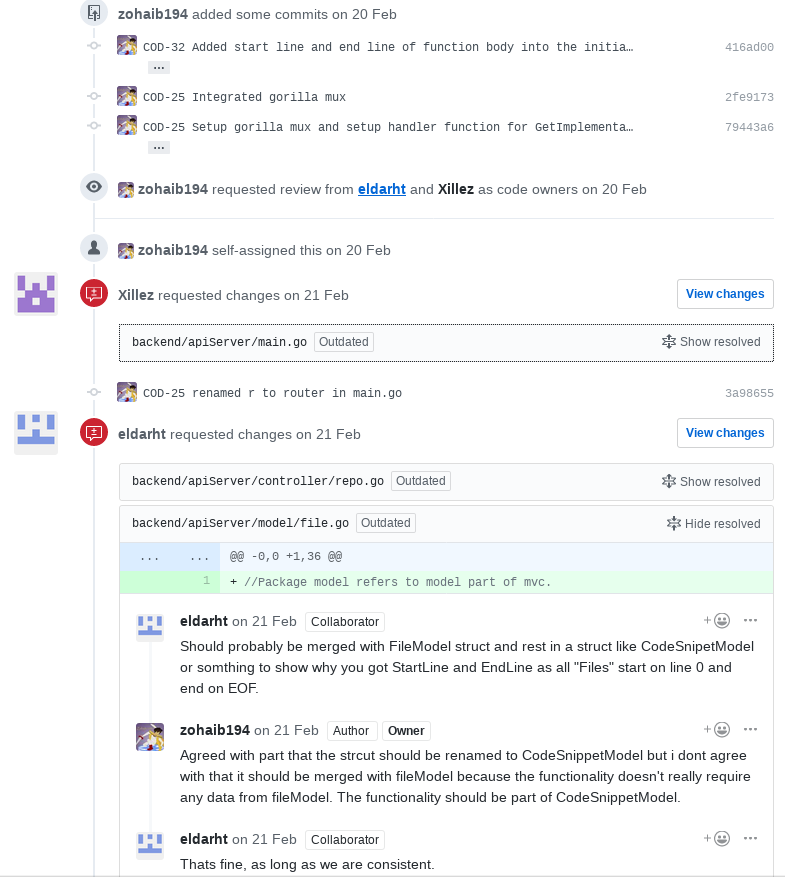
\includegraphics[width=\textwidth]{inc/images/pullrequestDiscussion.png}
    \noindent\rule{\textwidth}{1pt}
    \caption{Pull request discussion.}
    \label{fig:pullrequestDiscussion}
\end{figure}

Project status was documented with \gls{jira}, \gls{confluence} and \gls{git}.

Mondays were used for meetings and started off by having a meeting with supervisor followed by preparation for meeting with product owner, then said meeting and ended with retrospective meeting or internal meetings.

\subsubsection{Meetings with supervisor}
\newglossaryentry{reviewMeeting}{name={review meeting}, description={A process where \gls{scrum} team shows what was accomplished during the \gls{sprint} \cite{schwaberScrum.2017}}}
Meetings with supervisor were used as a \gls{sprint} \gls{reviewMeeting}, discussing what was completed or not in the last \gls{sprint}, and how the team worked. Suggestions on how to improve the development process or documentation and professionalism were given to the team.  

\subsubsection{Meetings with product owner}

\newglossaryentry{backlog}{name={product backlog}, description={An ordered list of everything that is known to be needed in the product \cite{schwaberScrum.2017}}}
\newglossaryentry{sprintbacklog}{name={sprint backlog}, description={Set of \gls{backlog} items selected for the \gls{sprint} \cite{schwaberScrum.2017}}}
\newglossaryentry{softwaredesignpattern}{name={software design pattern}, description={A reusable solution to a commonly occurring problem within a given context in software design}}
\newglossaryentry{planningMeeting}{name={planning meeting}, description={A process where product owner describes highest priority feature to the team}}

Planning for the meeting with product owner consisted of preparing a suggestion for a \gls{sprintbacklog}. The meetings were used as \gls{sprint} \gls{reviewMeeting} and \gls{sprint} \gls{planningMeeting}. General recommendations were given as well as specific recommendations on choice of technology or \gls{softwaredesignpattern}. The suggested \gls{sprintbacklog} was looked over and finalized according to product owner's input. 

\subsubsection{Internal meetings}
\newglossaryentry{sprintretrospective}{name={sprint retrospective}, description={Meeting for planning improvements to be enacted during the next \gls{sprint} \cite{schwaberScrum.2017}}}
Internal meetings were used for \gls{sprintretrospective} meetings and for story point estimation of the upcoming \gls{sprint}. 

\subsubsection{Story points}
\newglossaryentry{storypoint}{name={story point}, description={ An abstract measure of effort required to implement a user story}}

\begin{figure}[H]
    \noindent\rule{\textwidth}{1pt}    
    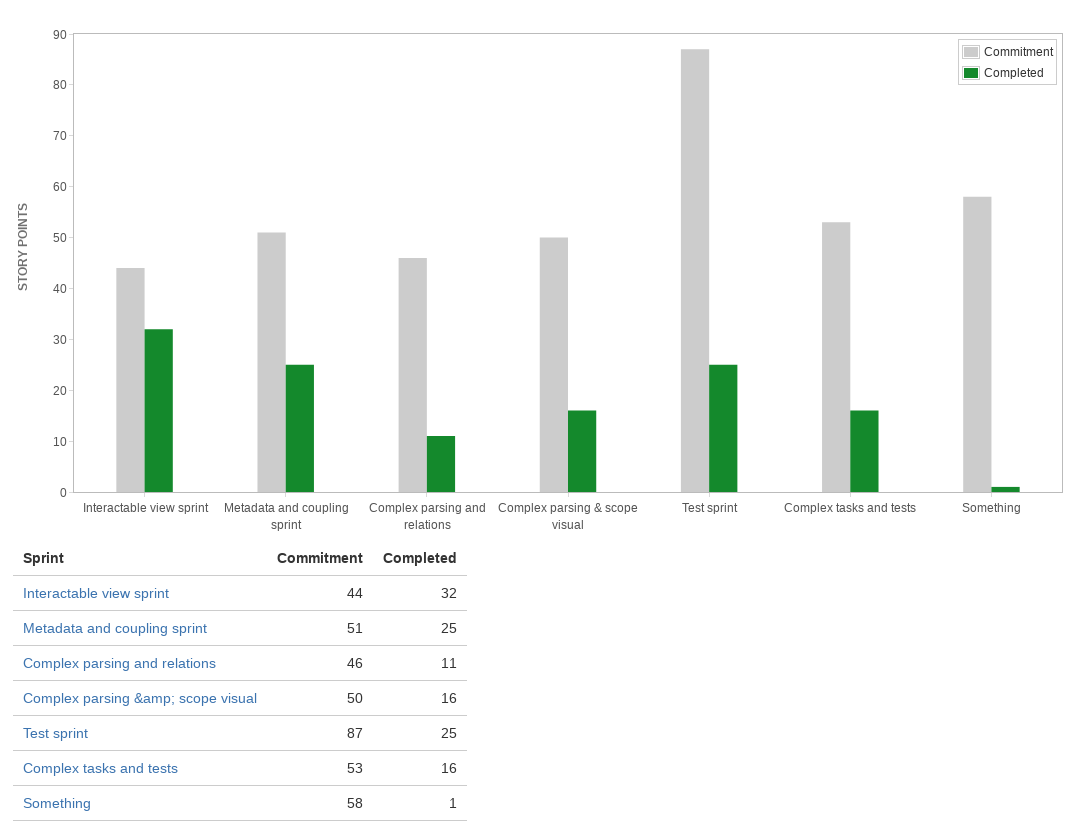
\includegraphics[width=\textwidth]{inc/images/velocity.png}
    \noindent\rule{\textwidth}{1pt}
    \caption{Velocity chart.}
    \label{fig:velocityChart}
\end{figure}

For estimation \glspl{storypoint} were used. \Glspl{storypoint} were given based on relative size, and time value changed over time. This change meant that the teams velocity as shown in figure \ref{fig:velocityChart} is misleading.

\subsubsection{Scrum board}
\begin{figure}[H]
    \noindent\rule{\textwidth}{1pt}    
    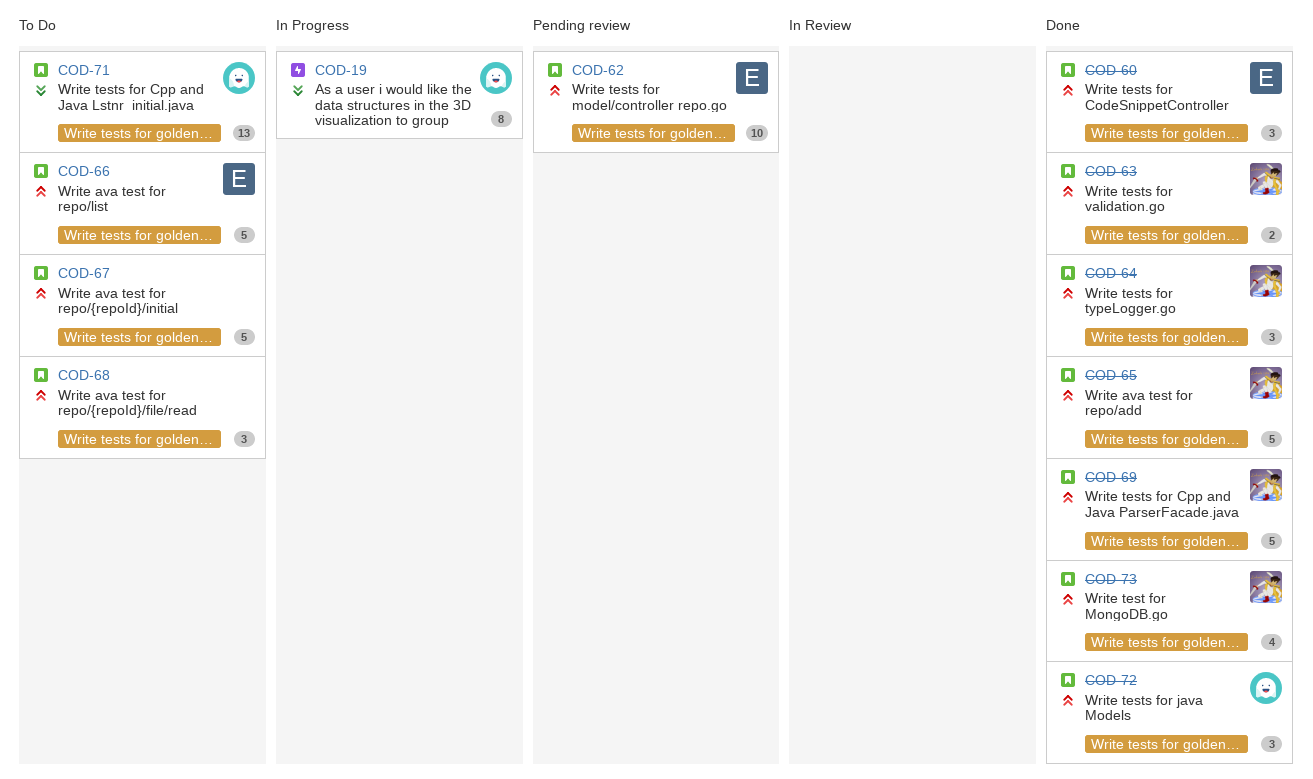
\includegraphics[width=\textwidth]{inc/images/board.png}
    \noindent\rule{\textwidth}{1pt}
    \caption{Scrum board for test sprint.}
    \label{fig:scrumBoar}
\end{figure}

As shown in figure \ref{fig:scrumBoar}, the workflow was divided into five parts:

\begin{itemize}
    \item "To Do" - \Gls{sprintbacklog}.
    \item "In Progress" - Tasks currently being worked on.
    \item "Pending review" - Developer consider the task completed and want other team members to review it.
    \item "In Review" - Team member has reviewed task and requested changes.
    \item "Done" - Team members have accepted and merged pull request.
\end{itemize}

\section{Sprint Overview}
\newglossaryentry{burndown}{name={burndown}, description={A graphical representation of work left to do versus time \cite{wiki:burndown}}}
\subsection{Sprint: hello world (02. feb - 13. feb)}
\begin{figure}[H] 
    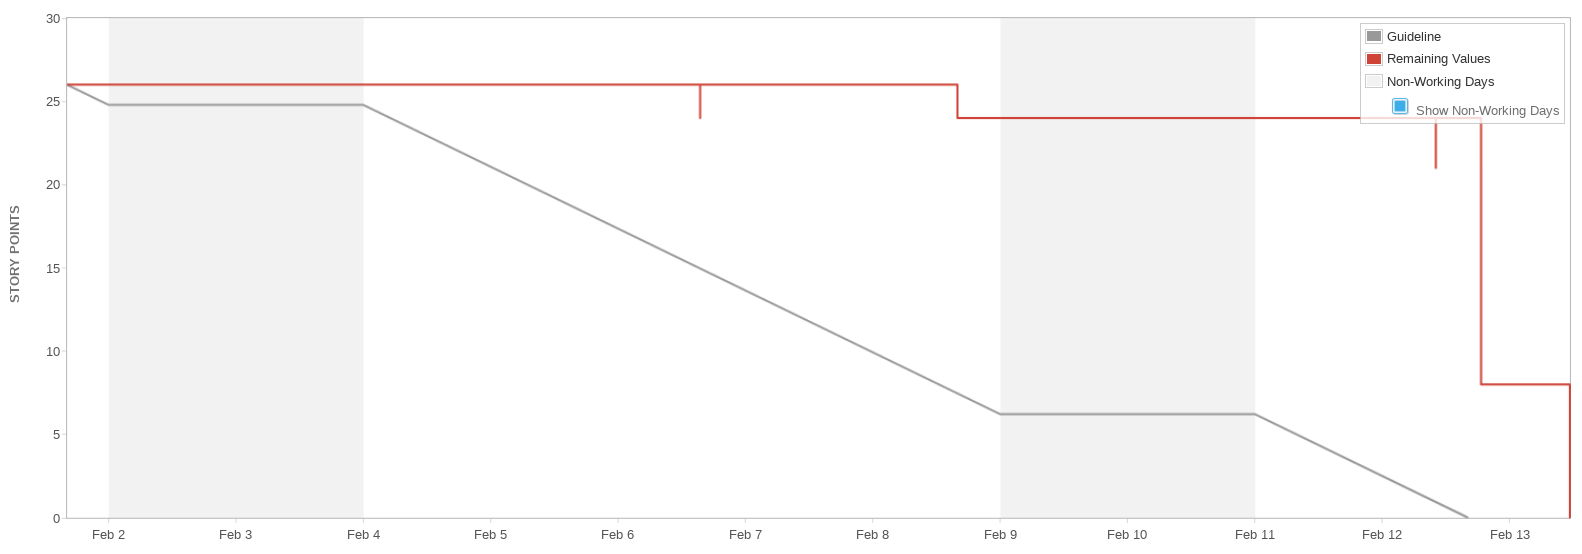
\includegraphics[width=\textwidth]{inc/images/sprints/sprintHelloWorld020219-130219.png}
    \caption{\Gls{burndown} chart for \gls{sprint} hello world.}
    \label{fig:sprintHellWorld}
\end{figure}

\newacronym{uri}{URI}{Uniform Resource Identifier}
\newglossaryentry{frontend}{name={front-end}, description={The presentation layer of a software}}
\newacronym{rest}{REST}{REpresentational State Transfer}
\newglossaryentry{webgl}{name={WebGL}, description={A JavaScript API for rendering interactive 2D and 3D graphics within any compatible web browser without the use of plug-ins \cite{wiki:webgl}}}


In this sprint the idea was to make a prototype that could represent a function definition from a \gls{git} repository \gls{uri}. The prototype should also indicate to the user if the browser does not support \gls{webgl}.

As figure \ref{fig:sprintHellWorld} shows, sprint took more time to finish than planned. The reason was that it took some time to get the parsed code to follow the planned \gls{json} format. This led to delays in visualizing it in the \gls{frontend}. \Gls{json} was a blocker for merging, once this was done all remaining task were completed.

\subsubsection{Front-end}
In \gls{frontend}, two \gls{html} pages were partially implemented; home page and visualization page.
In the homepage a field for submitting the \gls{git} repository link was created. If a valid repository \gls{uri} was submitted, user would be redirected to visualization page where loading would be shown. Once loading was completed a 3D visualization would be presented to the user.
There a representation of simple functions with random placement in 3D environment was implemented.

\subsubsection{Back-end}
In the \gls{backend}, \gls{api} \gls{rest} endpoints for initial request and adding \gls{git} repository link to database was implemented, along with java parsing for parts of simple function definitions. 

\subsection{Sprint: representation of complex data (14. feb - 18. feb)}
\begin{figure}[H] 
    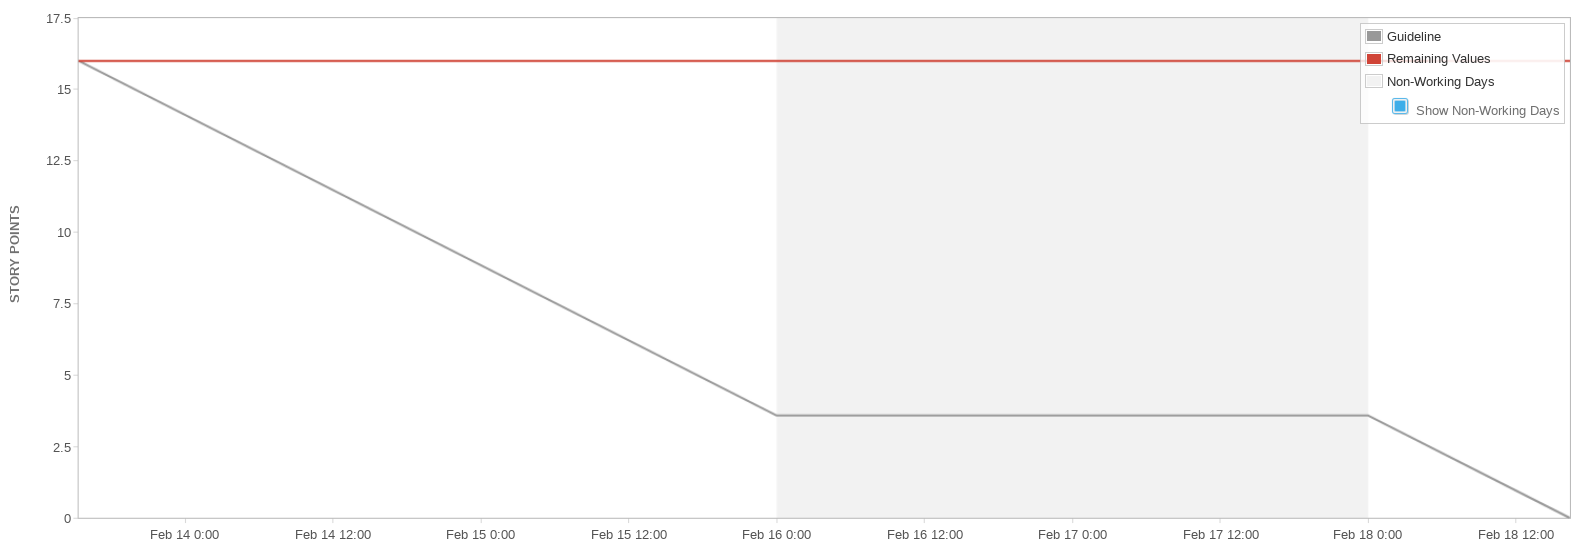
\includegraphics[width=\textwidth]{inc/images/sprints/sprintRepresentComplexData140219-180219.png}
    \caption{\Gls{burndown} chart for \gls{sprint} representation of complex data.}
    \label{fig:sprintRepresentationOfComplexData}
\end{figure}
\newacronym{gui}{GUI}{Graphical User \Gls{interface}}
\newglossaryentry{sourcecode}{name={source code}, description={Any collection of code, possibly with comments, written using a human-readable programming language, usually as plain text \cite{wiki:sourceCode}}}
The goal of the \gls{sprint} was to relate the visualization structure to its \gls{sourcecode} implementation and group together related structures.

Unfortunately no tasks were fully completed and all got transferred to the next \gls{sprint}. This is the reason for why the Actual Work Remaining line in Figure \ref{fig:sprintRepresentationOfComplexData} doesn't decrease within this \gls{sprint}. The tasks were underestimated and far too large to be completed.

\subsubsection{Front-end}
In the \gls{frontend}, the \gls{gui} for data structure implementation was failed to be integrated. Requirements for fulfilling this task were not satisfied. Therefore updating \gls{backend} was prioritized.
A basic version of \gls{fdg} that handles parenting relations of data structures was implemented but wasn't considered complete. \Glspl{namespace} were also only partially implemented.

\subsubsection{Back-end}
In the \gls{backend}, \gls{jap} was updated for function definition \gls{json} to include start line and end line for fetching its implementation. \Glspl{namespace} were also parsed.


\subsection{Sprint: interactable (20. feb - 25. feb)}
\begin{figure}[H] 
    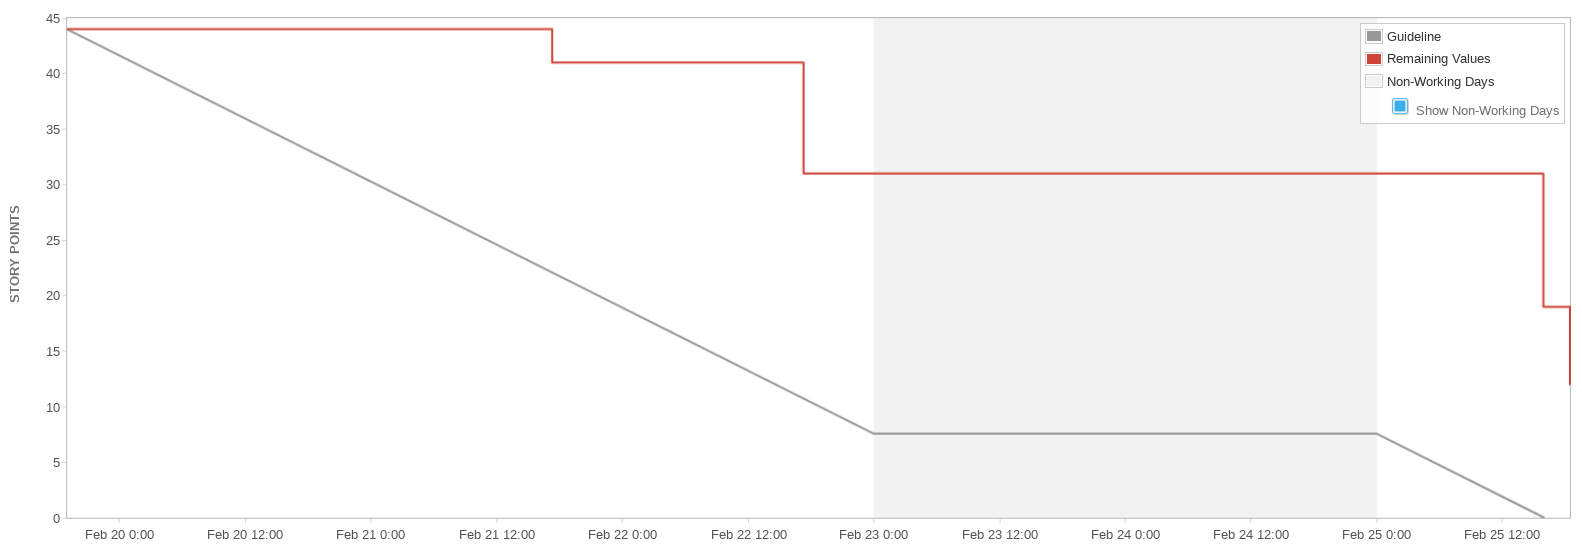
\includegraphics[width=\textwidth]{inc/images/sprints/sprintInteractable200219-250219.png}
    \caption{\Gls{burndown} chart for \gls{sprint} interactable.}
    \label{fig:sprintInteractable}
\end{figure}
The goal of this \gls{sprint} was to finish previous sprint, along with research on how to use \gls{antlr} for scope parsing. To improve on the previous \gls{sprint}, the tasks were divided more finely and declared more clearly.

\subsubsection{Front-end}
In the \gls{frontend}, the \gls{gui} layout of the system was implemented on the visualization page. Minor refactoring on \gls{frontend} was also done during this \gls{sprint}.

\subsubsection{Back-end}
In the \gls{backend}, was updated with a new \gls{api} endpoint for fetching implementation of functions. For \gls{jap}, through research the team found a recommended way to parse scopes from codebase using stack data structure \cite{parr2013definitive}. The task was underestimated and took some extra time to integrate the new implementation in \gls{jap}.

\subsection{Sprint: metadata and coupling (26. feb - 04. mar)}
\newglossaryentry{epic}{name={epic}, description={Large bodies of work that can be broken down into a number of smaller tasks \cite{atlassian:epic}}}
\begin{figure}[H] 
    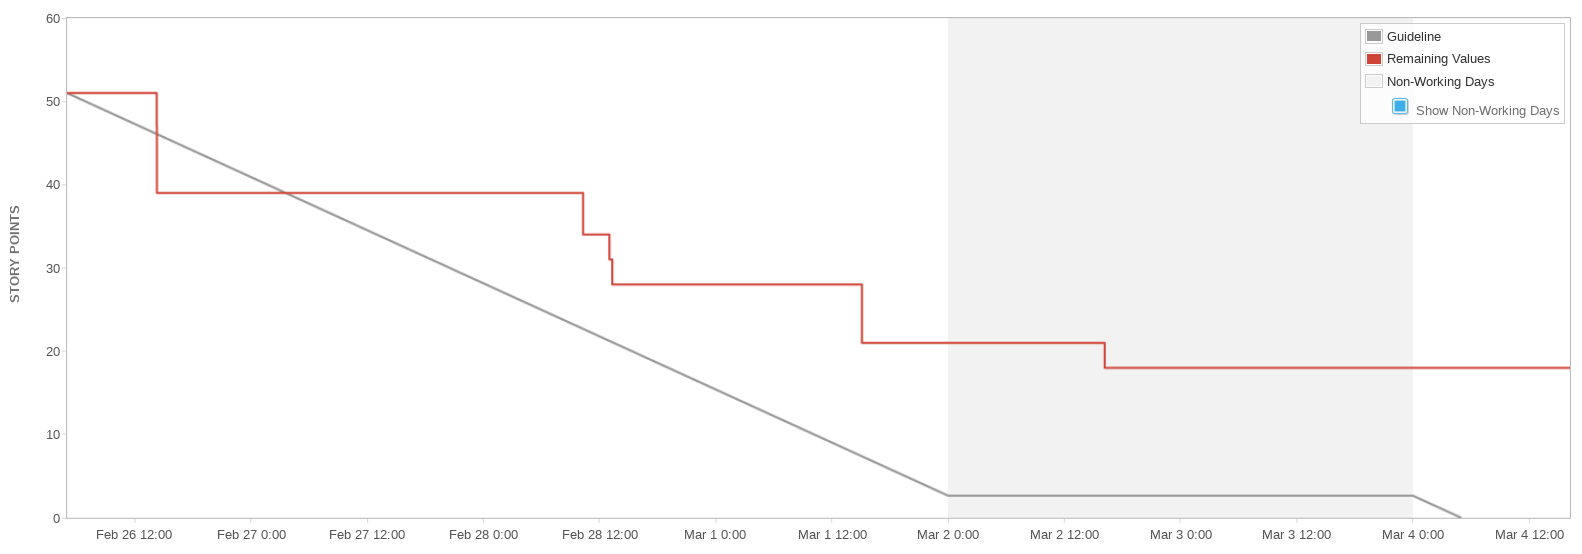
\includegraphics[width=\textwidth]{inc/images/sprints/sprintMetaData260219-040319.png}
    \caption{\Gls{burndown} chart for \gls{sprint} metadata and coupling.}
    \label{fig:sprintMetaDataAndCoupling}
\end{figure}
The goal of this \gls{sprint} was to add data about the project into the representation and visualize function calls.

Figure \ref{fig:sprintMetaDataAndCoupling} is a little misleading since it shows that the team was ahead of Ideal Work Remaining line. The reason Actual Work Remaining line dropped was that a task that should not have been in this \gls{sprint} was removed. From the previous \gls{sprint} the team also noticed that many tasks were \gls{fullstack} tasks and took a lot of time to finish. In this \gls{sprint} the team made \gls{fullstack} tasks into \glspl{epic}, divided them into stories and added sub-tasks under them so that the progress of the \gls{sprint} seemed continuous. The team also missed estimating sub-tasks which would have made the \gls{burndown} chart look even smoother. 

Some of the tasks in this \gls{sprint} were still big and depended on other tasks. Tasks such as display function calls was a very difficult \gls{fullstack} task that existed throughout all \glspl{sprint}. 

\subsubsection{Front-end}
In the \gls{frontend}, the team was able to connect the implementation window to show the implementation of simple function once clicked. Quality metrics window was also updated with simple metrics such as \gls{loc}, number of functions, classes and \glspl{namespace}. Repository window was implemented to show the repositories stored in the database, along with a \gls{rest} \gls{api} endpoint to fetch repositories.

\subsubsection{Back-end}
In the \gls{backend}, initial request functionality was updated to use \glspl{websocket}. This was done due to lack of information on processing of project files for the user on the loading page. Scope sensitive parsing was properly integrated in \gls{jap}.

\subsection{Sprint: complex parsing and relation (05. mar - 11. mar)}
\begin{figure}[H] 
    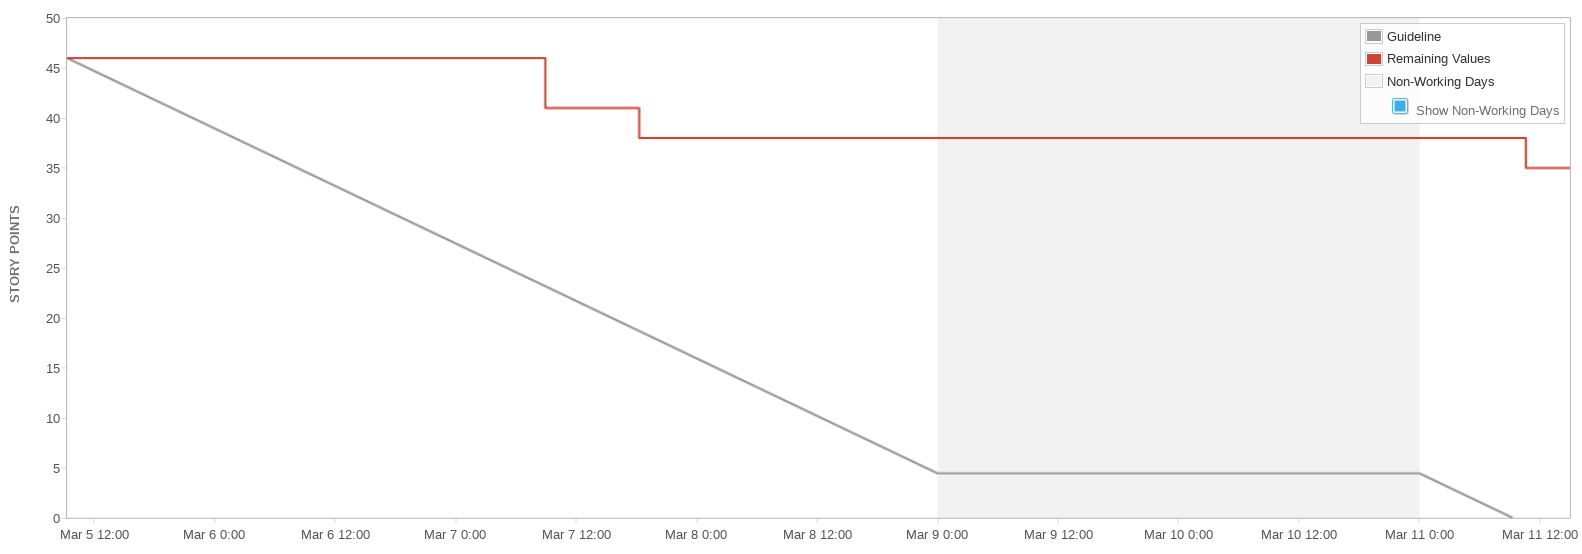
\includegraphics[width=\textwidth]{inc/images/sprints/sprintComplexParsingandRelation050319-110319.png}
    \caption{Burndown chart for sprint complex parsing and relation.}
    \label{fig:sprintComplexParsingAndRelation}
\end{figure}

The goal of this \gls{sprint} was to parse classes and continue improving parsing for function calls, in addition to research on quality metrics and measures.

\subsubsection{Front-end}
In the \gls{frontend}, the home page was updated with information on features completeness, browser support and contact information.

\subsubsection{Back-end}
In the \gls{backend}, \gls{websocket} was implemented.

The following were partially implemented or touched briefly due to other tasks having priority, which were too large and underestimated:
\begin{itemize}
    \item Parsing of classes for visualization.
    \item Parsing and extension of \gls{api} to include function calls for connecting related functions and classes.
    \item Research on complexity measures and applications/services that could perform these measures.
    \item View of implementation of functions.
\end{itemize}

This is also reflected in figure \ref{fig:sprintComplexParsingAndRelation}.

\subsection{Sprint: complex parsing and scope visual (12. mar - 18. mar)}     \label{subsection:SprintComplexParsingAndScopeVisual}
\begin{figure}[H] 
    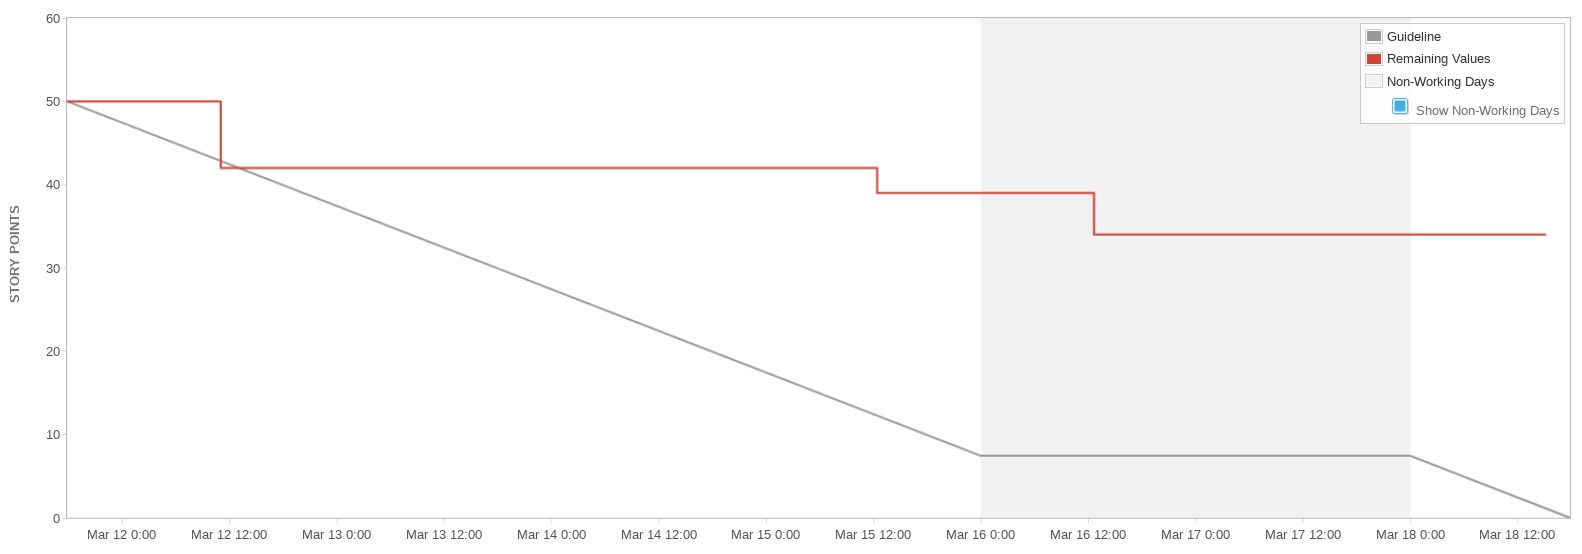
\includegraphics[width=\textwidth]{inc/images/sprints/sprintComplexParsingAndScopeVisual120319-180319.png}
    \caption{Burndown chart for sprint complex parsing and scope visual.}
    \label{fig:sprintComplexParsingAndScopeVisual}
\end{figure}
\newglossaryentry{planningPoker}{name={planning poker}, description={A consensus-based, gamified technique for estimating \cite{wiki:planningPoker}}}
\newglossaryentry{coupling}{name={coupling}, description={Is the degree of interdependence between software modules \cite{wiki:coupling}}}
\newglossaryentry{connacensemetrics}{name={connacense metrics}, description={A complexity measure for describing \gls{coupling} within a program}}
\newglossaryentry{cyclomaticcomplexity}{name={cyclomatic complexity},description={A complexity metric based on number of conditional or paths through a program}}
\newglossaryentry{halstedcomplexity}{name={halsted complexity},description={A complexity metric based on number of Operands, Operators and the total number of usages of each of these}}
\newglossaryentry{sonarqube}{name={SonarQube}, description={An open source platform to perform automatic reviews with static analysis \cite{sonarqube_2008}}}

The goal of this \gls{sprint} was to continue parsing function calls and visualize data structures within their respective scope.

As figure \ref{fig:sprintComplexParsingAndScopeVisual} shows, some tasks took very long to finish. This was due to underestimation as it was hard to conceptualize all aspects of the task during the \gls{planningPoker} session. This \gls{sprint} was one of the longest \glspl{sprint} the team went through, in total the team spent over 200 hours. The reason for this was that the team was extensively behind schedule and many of the core functionalities had yet to be figured out.

\subsubsection{Front-end}
In the \gls{frontend}, tree structures were used instead of arrays for \gls{fdg}. Implementation of tree structure was required before visualization of scopes could be done.
\subsubsection{Back-end}
In the \gls{backend}, Go \gls{api} endpoint for initial request was updated to give information about function calls. A custom logger was implemented in Go \gls{api}. Research on different quality metrics such as \Gls{connacensemetrics}, \Gls{cyclomaticcomplexity} and \Gls{halstedcomplexity} was done, along with finding an existing solution that could do static analysis on a specified code block. The team was recommended by supervisor to look into \gls{sonarqube} \gls{api}. This would have worked for our purpose but it would require a lot of configuration and was not done due to prioritization and time limitations. 
There was a lot of refactoring done in this \gls{sprint}. In \gls{jap} more listeners provided by \gls{antlr} were used instead of huge nested if statement blocks.  Parsing classes and function calls were partially implemented, but took multiple \glspl{sprint} to finish due to the flexibility of C++. The reason function calls took too long to finish is explained in more details in appendix \ref{appendix:retrospective2019-03-18}.

\subsection{Sprint: testing (19. mar - 02. apr)}
\begin{figure}[H] 
    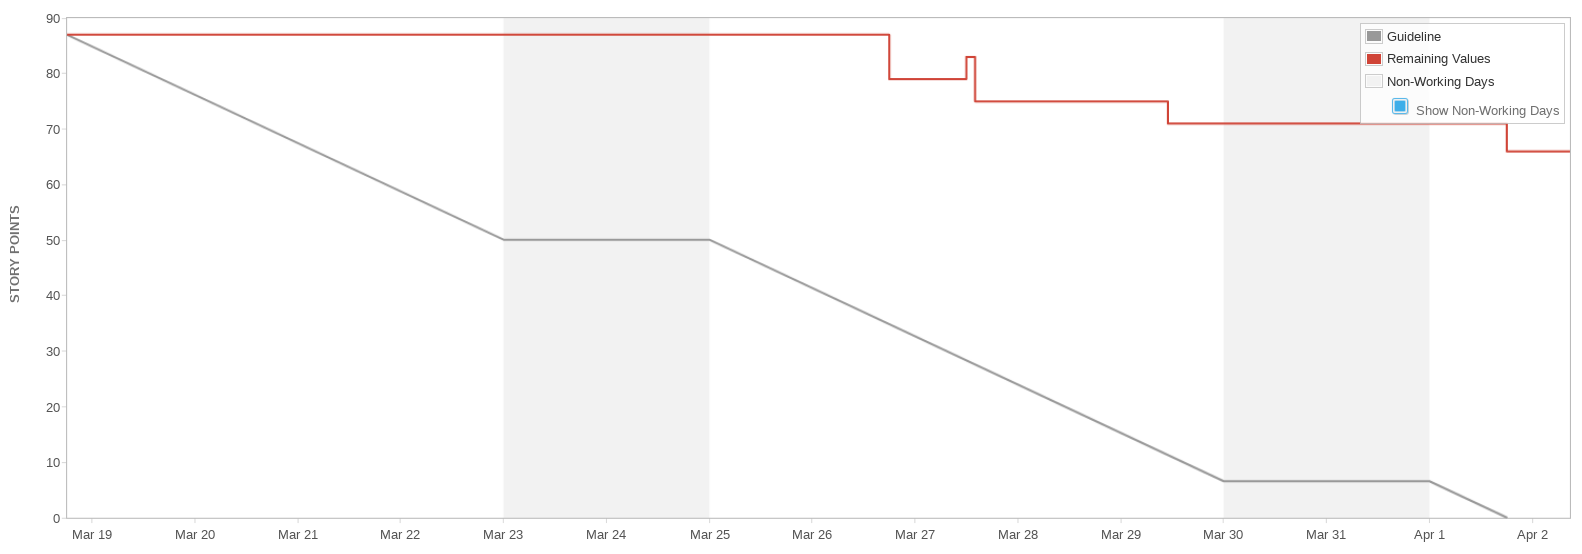
\includegraphics[width=\textwidth]{inc/images/sprints/sprintTest190319-020419.png}
    \caption{Burndown chart for sprint testing.}
    \label{fig:sprintTesting}
\end{figure}

\newglossaryentry{ava}{name={AVA}, description={Futuristic JavaScript test runner \cite{github:ava}}}
\newglossaryentry{junit}{name={JUnit}, description={A simple framework to write repeatable tests \cite{maven:junit}}}
This \gls{sprint} had a primary focus on testing and since no testing had been done and there were a lot of tests to write. Therefore it was decided to make this a two weeks long \gls{sprint}.

As the figure \ref{fig:sprintTesting} shows, no task was done in the first week and this is due to no experience with any of the testing framework that were used in this project such as \gls{junit} and \gls{ava}. 

\subsubsection{Back-end}
Tests in \gls{backend} were written for the following files and functionalities.
\begin{itemize}
    \item CodeSnippetController.go
    \item validation.go
    \item typeLogger.go
    \item repo/add - \gls{api}-endpoint
    \item Cpp and Java ParserFacade.java
    \item java Models
    \item MongoDB.go
\end{itemize}

\subsection{Sprint: complex task and testing (02. apr - 08. apr)}
\begin{figure}[H] 
    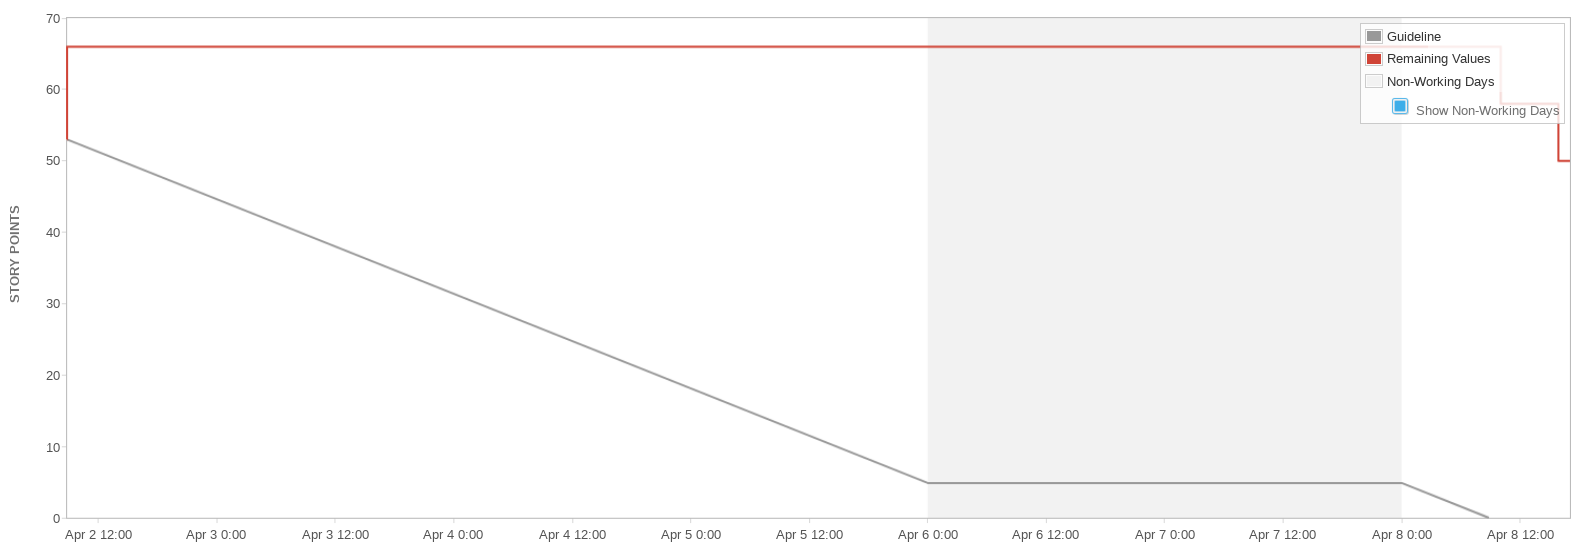
\includegraphics[width=\textwidth]{inc/images/sprints/sprintComplexTaskAndTest020419-080419.png}
    \caption{Burndown chart for sprint complex task and testing.}
    \label{fig:sprintComplexTaskAndTesting}
\end{figure}

This \gls{sprint} was a pair programming \gls{sprint} for tasks that were complicated and had existed throughout many \glspl{sprint}. Pair programming was very beneficial to get every group member up to date with the different components of the system that were initially implemented individually.
As the figure \ref{fig:sprintComplexTaskAndTesting} shows, it still took very long before the team could finish any task. This is due to the tasks in this \gls{sprint} being dependent on each other. The tasks were partially done before the team moved over to the dependent task and not finished before the end.
This made the pull request so large that the team were not able to accept it before the \gls{sprint} was completed.
Pair programming helped to get following task done;
\begin{itemize}
    \item In \gls{backend}, the \gls{jap} was updated with a complete implementation of class parsing, along with function calls parsing. 
    \item In \gls{frontend}, the visualization was updated with scopes inside scopes.
\end{itemize}

By the end of the \gls{sprint} some members felt that their time was better spent on individual tasks rather than pair programming.